\documentclass[a4paper]{article}

\def\npart {IB}
\def\nterm {Michaelmas}
\def\nyear {2015}
\def\nlecturer {G. R. Grimmett}
\def\ncourse {Markov Chains}
\def\nlectures {TT.10}
\def\nnotready {}

% Imports
\ifx \nextra \undefined
  \usepackage[pdftex,
    hidelinks,
    pdfauthor={Dexter Chua},
    pdfsubject={Cambridge Maths Notes: Part \npart\ - \ncourse},
    pdftitle={Part \npart\ - \ncourse},
  pdfkeywords={Cambridge Mathematics Maths Math \npart\ \nterm\ \nyear\ \ncourse}]{hyperref}
  \title{Part \npart\ - \ncourse}
\else
  \usepackage[pdftex,
    hidelinks,
    pdfauthor={Dexter Chua},
    pdfsubject={Cambridge Maths Notes: Part \npart\ - \ncourse\ (\nextra)},
    pdftitle={Part \npart\ - \ncourse\ (\nextra)},
  pdfkeywords={Cambridge Mathematics Maths Math \npart\ \nterm\ \nyear\ \ncourse\ \nextra}]{hyperref}

  \title{Part \npart\ - \ncourse \\ {\Large \nextra}}
\fi

\author{Lectured by \nlecturer \\\small Notes taken by Dexter Chua}
\date{\nterm\ \nyear}

\usepackage{alltt}
\usepackage{amsfonts}
\usepackage{amsmath}
\usepackage{amssymb}
\usepackage{amsthm}
\usepackage{booktabs}
\usepackage{caption}
\usepackage{enumitem}
\usepackage{fancyhdr}
\usepackage{graphicx}
\usepackage{mathtools}
\usepackage{microtype}
\usepackage{multirow}
\usepackage{pdflscape}
\usepackage{pgfplots}
\usepackage{siunitx}
\usepackage{tabularx}
\usepackage{tikz}
\usepackage{tkz-euclide}
\usepackage[normalem]{ulem}
\usepackage[all]{xy}

\pgfplotsset{compat=1.12}

\pagestyle{fancyplain}
\lhead{\emph{\nouppercase{\leftmark}}}
\ifx \nextra \undefined
  \rhead{
    \ifnum\thepage=1
    \else
      \npart\ \ncourse
    \fi}
\else
  \rhead{
    \ifnum\thepage=1
    \else
      \npart\ \ncourse\ (\nextra)
    \fi}
\fi
\usetikzlibrary{arrows}
\usetikzlibrary{decorations.markings}
\usetikzlibrary{decorations.pathmorphing}
\usetikzlibrary{positioning}
\usetikzlibrary{fadings}
\usetikzlibrary{intersections}
\usetikzlibrary{cd}

\newcommand*{\Cdot}{\raisebox{-0.25ex}{\scalebox{1.5}{$\cdot$}}}
\newcommand {\pd}[2][ ]{
  \ifx #1 { }
    \frac{\partial}{\partial #2}
  \else
    \frac{\partial^{#1}}{\partial #2^{#1}}
  \fi
}

% Theorems
\theoremstyle{definition}
\newtheorem*{aim}{Aim}
\newtheorem*{axiom}{Axiom}
\newtheorem*{claim}{Claim}
\newtheorem*{cor}{Corollary}
\newtheorem*{defi}{Definition}
\newtheorem*{eg}{Example}
\newtheorem*{fact}{Fact}
\newtheorem*{law}{Law}
\newtheorem*{lemma}{Lemma}
\newtheorem*{notation}{Notation}
\newtheorem*{prop}{Proposition}
\newtheorem*{thm}{Theorem}

\renewcommand{\labelitemi}{--}
\renewcommand{\labelitemii}{$\circ$}
\renewcommand{\labelenumi}{(\roman{*})}

\let\stdsection\section
\renewcommand\section{\newpage\stdsection}

% Strike through
\def\st{\bgroup \ULdepth=-.55ex \ULset}

% Maths symbols
\newcommand{\bra}{\langle}
\newcommand{\ket}{\rangle}

\newcommand{\N}{\mathbb{N}}
\newcommand{\Z}{\mathbb{Z}}
\newcommand{\Q}{\mathbb{Q}}
\renewcommand{\H}{\mathbb{H}}
\newcommand{\R}{\mathbb{R}}
\newcommand{\C}{\mathbb{C}}
\newcommand{\Prob}{\mathbb{P}}
\renewcommand{\P}{\mathbb{P}}
\newcommand{\E}{\mathbb{E}}
\newcommand{\F}{\mathbb{F}}
\newcommand{\cU}{\mathcal{U}}
\newcommand{\RP}{\mathbb{RP}}
\newcommand{\CP}{\mathbb{CP}}

\newcommand{\ph}{\,\cdot\,}

\DeclareMathOperator{\sech}{sech}
\DeclareMathOperator{\cosech}{cosech}
\DeclareMathOperator{\cosec}{cosec}

\DeclareMathOperator{\covol}{covol}
\DeclareMathOperator{\vol}{vol}

\let\Im\relax
\let\Re\relax
\DeclareMathOperator{\Im}{Im}
\DeclareMathOperator{\Re}{Re}
\DeclareMathOperator{\im}{im}
\DeclareMathOperator{\image}{image}
\DeclareMathOperator{\Ann}{Ann}

\DeclareMathOperator*{\res}{res}
\DeclareMathOperator{\Res}{Res}
\DeclareMathOperator{\Ind}{Ind}

\DeclareMathOperator{\tr}{tr}
\DeclareMathOperator{\diag}{diag}
\DeclareMathOperator{\rank}{rank}
\DeclareMathOperator{\card}{card}
\DeclareMathOperator{\spn}{span}
\DeclareMathOperator{\adj}{adj}

\DeclareMathOperator{\erf}{erf}
\DeclareMathOperator{\erfc}{erfc}

\DeclareMathOperator{\ord}{ord}
\DeclareMathOperator{\Sym}{Sym}

\DeclareMathOperator{\sgn}{sgn}
\DeclareMathOperator{\orb}{orb}
\DeclareMathOperator{\stab}{stab}
\DeclareMathOperator{\ccl}{ccl}

\DeclareMathOperator{\lcm}{lcm}
\DeclareMathOperator{\hcf}{hcf}

\DeclareMathOperator{\Int}{Int}
\DeclareMathOperator{\id}{id}

\DeclareMathOperator{\betaD}{beta}
\DeclareMathOperator{\gammaD}{gamma}
\DeclareMathOperator{\Poisson}{Poisson}
\DeclareMathOperator{\binomial}{binomial}
\DeclareMathOperator{\multinomial}{multinomial}
\DeclareMathOperator{\Bernoulli}{Bernoulli}
\DeclareMathOperator{\like}{like}

\DeclareMathOperator{\var}{var}
\DeclareMathOperator{\cov}{cov}
\DeclareMathOperator{\bias}{bias}
\DeclareMathOperator{\mse}{mse}
\DeclareMathOperator{\corr}{corr}

\DeclareMathOperator{\otp}{otp}
\DeclareMathOperator{\dom}{dom}

\DeclareMathOperator{\Root}{Root}
\DeclareMathOperator{\supp}{supp}
\DeclareMathOperator{\rel}{rel}
\DeclareMathOperator{\Hom}{Hom}
\DeclareMathOperator{\Aut}{Aut}
\DeclareMathOperator{\Gal}{Gal}
\DeclareMathOperator{\Mat}{Mat}
\DeclareMathOperator{\End}{End}
\DeclareMathOperator{\Char}{char}
\DeclareMathOperator{\ev}{ev}
\DeclareMathOperator{\St}{St}
\DeclareMathOperator{\Lk}{Lk}
\DeclareMathOperator{\disc}{disc}
\DeclareMathOperator{\Isom}{Isom}
\DeclareMathOperator{\length}{length}
\DeclareMathOperator{\energy}{energy}
\DeclareMathOperator{\area}{area}
\DeclareMathOperator{\Syl}{Syl}
\DeclareMathOperator{\cl}{cl}
\DeclareMathOperator{\fix}{fix}

\newcommand{\GL}{\mathrm{GL}}
\newcommand{\SL}{\mathrm{SL}}
\newcommand{\PGL}{\mathrm{PGL}}
\newcommand{\PSL}{\mathrm{PSL}}
\newcommand{\PSU}{\mathrm{PSU}}
\newcommand{\Or}{\mathrm{O}}
\newcommand{\SO}{\mathrm{SO}}
\newcommand{\U}{\mathrm{U}}
\newcommand{\SU}{\mathrm{SU}}

\renewcommand{\d}{\mathrm{d}}
\newcommand{\D}{\mathrm{D}}

\tikzset{->/.style = {decoration={markings,
                                  mark=at position 1 with {\arrow[scale=2]{latex'}}},
                      postaction={decorate}}}
\tikzset{<-/.style = {decoration={markings,
                                  mark=at position 0 with {\arrowreversed[scale=2]{latex'}}},
                      postaction={decorate}}}
\tikzset{<->/.style = {decoration={markings,
                                   mark=at position 0 with {\arrowreversed[scale=2]{latex'}},
                                   mark=at position 1 with {\arrow[scale=2]{latex'}}},
                       postaction={decorate}}}
\tikzset{->-/.style = {decoration={markings,
                                   mark=at position #1 with {\arrow[scale=2]{latex'}}},
                       postaction={decorate}}}
\tikzset{-<-/.style = {decoration={markings,
                                   mark=at position #1 with {\arrowreversed[scale=2]{latex'}}},
                       postaction={decorate}}}

\tikzset{circ/.style = {fill, circle, inner sep = 0, minimum size = 3}}
\tikzset{mstate/.style={circle, draw, blue, text=black, minimum width=0.7cm}}

\definecolor{mblue}{rgb}{0.2, 0.3, 0.8}
\definecolor{morange}{rgb}{1, 0.5, 0}
\definecolor{mgreen}{rgb}{0.1, 0.4, 0.2}
\definecolor{mred}{rgb}{0.5, 0, 0}

\def\drawcirculararc(#1,#2)(#3,#4)(#5,#6){%
    \pgfmathsetmacro\cA{(#1*#1+#2*#2-#3*#3-#4*#4)/2}%
    \pgfmathsetmacro\cB{(#1*#1+#2*#2-#5*#5-#6*#6)/2}%
    \pgfmathsetmacro\cy{(\cB*(#1-#3)-\cA*(#1-#5))/%
                        ((#2-#6)*(#1-#3)-(#2-#4)*(#1-#5))}%
    \pgfmathsetmacro\cx{(\cA-\cy*(#2-#4))/(#1-#3)}%
    \pgfmathsetmacro\cr{sqrt((#1-\cx)*(#1-\cx)+(#2-\cy)*(#2-\cy))}%
    \pgfmathsetmacro\cA{atan2(#2-\cy,#1-\cx)}%
    \pgfmathsetmacro\cB{atan2(#6-\cy,#5-\cx)}%
    \pgfmathparse{\cB<\cA}%
    \ifnum\pgfmathresult=1
        \pgfmathsetmacro\cB{\cB+360}%
    \fi
    \draw (#1,#2) arc (\cA:\cB:\cr);%
}
\newcommand\getCoord[3]{\newdimen{#1}\newdimen{#2}\pgfextractx{#1}{\pgfpointanchor{#3}{center}}\pgfextracty{#2}{\pgfpointanchor{#3}{center}}}

\def\Xint#1{\mathchoice
   {\XXint\displaystyle\textstyle{#1}}%
   {\XXint\textstyle\scriptstyle{#1}}%
   {\XXint\scriptstyle\scriptscriptstyle{#1}}%
   {\XXint\scriptscriptstyle\scriptscriptstyle{#1}}%
   \!\int}
\def\XXint#1#2#3{{\setbox0=\hbox{$#1{#2#3}{\int}$}
     \vcenter{\hbox{$#2#3$}}\kern-.5\wd0}}
\def\ddashint{\Xint=}
\def\dashint{\Xint-}


\begin{document}
\maketitle
{\small
\noindent\textbf{Discrete-time chains}\\
Definition and basic properties, the transition matrix. Calculation of $n$-step transition probabilities. Communicating classes, closed classes, absorption, irreducibility. Calculation of hitting probabilities and mean hitting times; survival probability for birth and death chains. Stopping times and statement of the strong Markov property.\hspace*{\fill} [5]

\vspace{5pt}
\noindent Recurrence and transience; equivalence of transience and summability of $n$-step transition probabilities; equivalence of recurrence and certainty of return. Recurrence as a class property, relation with closed classes. Simple random walks in dimensions one, two and three.\hspace*{\fill} [3]

\vspace{5pt}
\noindent Invariant distributions, statement of existence and uniqueness up to constant multiples. Mean return time, positive recurrence; equivalence of positive recurrence and the existence of an invariant distribution. Convergence to equilibrium for irreducible, positive recurrent, aperiodic chains *and proof by coupling*. Long-run proportion of time spent in a given state.\hspace*{\fill} [3]

\vspace{5pt}
\noindent Time reversal, detailed balance, reversibility, random walk on a graph.\hspace*{\fill} [1]}

\tableofcontents
\setcounter{section}{-1}
\section{Introduction}
So far, in IA Probability, we have always dealt with one random variable, or numerous independent variables, and we were able to handle them. However, in real life, things often \emph{are} dependent, and things become much more difficult. There are many ways in which variables can be dependent. Their dependence can be very complicated, or very simple. We don't really know what to do with them.

This is similar to our study of functions. We can develop theories about continuous functions, increasing functions, or differentiable functions, but if we are just given a random function without assuming anything about it, there really isn't much we can do.

Hence, in this course, we are just going to study a particular kind of dependent variables. In fact, in IA Probability, we did encounter some of these. For example, we dealt with random walks, in which the next position depends on the previous position. This gives us some dependent random variables, but they are dependent in a very simple way.

In reality, a random walk is too simple of a model to describe the world. We need something more general, and these are known as \emph{Markov chains}. These are random distributions that satisfy the \emph{Markov assumption}. This assumption, intuitively, says that the future depends only upon the current state, and not how we got to the current state.

\section{The Markov property}
\begin{defi}[Markov chain]
  Let $\mathbf{X} = (X_0, X_1, \cdots)$ be a sequence of random variables taking values in some set $S$, the \emph{state space}. We assume that $S$ is countable (which could be finite). $\mathbf{X}$ has the \emph{Markov property} if
  \[
    \P(X_{n + 1} = i_{n + 1} | X_0 = i_0, \cdots, X_n = i_n) = \P(X_{n + 1} = i_{n + 1} | X_n = i_n)
  \]
  for all $n\geq 0, i_0,\cdots, i_{n + 1}\in S$.

  If $\mathbf{X}$ has the Markov property, we call it a \emph{Markov chain}.

  We say that a Markov chain $\mathbf{X}$ is \emph{homogeneous} if the conditional probabilities $\P(X_{n + 1} = j | X_n = i)$ do not depend on $n$.
\end{defi}
All our chains $\mathbf{X}$ will be Markov and homogeneous unless otherwise specified.

\begin{eg}\leavevmode
  \begin{enumerate}
    \item A random walk is a Markov chain.
    \item The branching process is a Markov chain.
  \end{enumerate}
\end{eg}

In general, to fully specify a (homogeneous) Markov chain, we will need two items:
\begin{enumerate}
  \item The initial distribution $\lambda_i = \P(X_0 = i)$. We can write this as a vector $\lambda = (\lambda_i: i \in S)$.
  \item The transition probabilities $p_{ij} = \P(X_{n + 1} = j | X_n = i)$. We can write this as a matrix $P = (p_{ij})_{i, j\in S}$.
\end{enumerate}

There are some preliminary properties we know about these items. They are what decide whether a pair $(\lambda, P)$ actually specify a Markov chain.
\begin{prop}\leavevmode
  \begin{enumerate}
    \item $\lambda$ is a \emph{distribution}, ie. $\lambda_i \geq 0, \sum_i \lambda_i = 1$.
    \item $P$ is a \emph{stochastic matrix}, ie. $p_{ij} \geq 0$ and $\sum_j p_{ij} = 1$ for all $i$.
  \end{enumerate}
\end{prop}

\begin{proof}\leavevmode
  \begin{enumerate}
    \item Obvious since $\lambda$ is a probability distribution.
    \item $p_{ij} \geq 0$ since $p_{ij}$ is a probability. We also have
      \[
        \sum_j p_{ij} = \sum_j \P(X_{1} = j | X_0 = i) = 1
      \]
      since $\P(X_1 = \ph | X_0 = i)$ is a probability distribution function.
  \end{enumerate}
\end{proof}
Note that we only require the row sum to be $1$, and the column sum need not be.

We will prove another seemingly obvious fact.
\begin{thm}
  Let $\lambda$ be a distribution (on $S$) and $P$ a stochastic matrix. The sequence $\mathbf{X} = (X_0, X_1, \cdots)$ is a Markov chain with initial distribution $\lambda$ and transition matrix $P$ iff
  \[
    \P(X_0 = i, X_1 = i_1, \cdots, X_n = i_n) = \lambda_{i_0}p_{i_0 i_1}p_{i_1i_2}\cdots p_{i_{n - 1}i_n}\tag{$*$}
  \]
  for all $n, i_0, \cdots, i_n$
\end{thm}
\begin{proof}
  Let $A_k$ be the event $X_k = i_k$. Then we can write $(*)$ as
  \[
    \P(A_0\cap A_1\cap\cdots \cap A_n) = \lambda_{i_0}p_{i_0 i_1}p_{i_1i_2}\cdots p_{i_{n - 1}i_n}. \tag{$*$}
  \]
  We first assume that $\mathbf{X}$ is a Markov chain. We prove $(*)$ by induction on $n$.

  When $n = 0$, $(*)$ says $\P(A_0) = \lambda_{i_0}$. This is true by definition of $\lambda$.

  Assume that it is true for all $n < N$. Then
  \begin{align*}
    \P(A_0 \cap A_1 \cap \cdots \cap A_N) &= \P(A_0,\cdots, A_{N - 1})\P(A_0, \cdots, A_n | A_0, \cdots, A_{N - 1})\\
    &= \lambda_{i_0} p_{i_0 i_1}\cdots p_{i_{N - 2}i_{N - 1}} \P(A_{N} | A_0,\cdots, A_{N - 1})\\
    &= \lambda_{i_0} p_{i_0 i_1}\cdots p_{i_{N - 2}i_{N - 1}} \P(A_{N} | A_{N - 1})\\
    &= \lambda_{i_0}p_{i_0 i_1}p_{i_1i_2}\cdots p_{i_{N - 1}i_N}.
  \end{align*}
  So it is true for $N$ as well. Hence we are done by induction.

  Conversely, suppose that ($*$) holds. Then for $n = 0$, we have $\P(X_0 = i_0) = \lambda_{i_0}$. Otherwise
  \begin{align*}
    \P(X_n = i_n| X_0 = i_0, \cdots, X_{n - 1} = i_{n - 1}) &= \P(A_n | A_0 \cap \cdots\cap A_{n - 1})\\
    &= \frac{\P(A_0\cap \cdots \cap A_n)}{\P(A_0\cap \cdots \cap A_{n - 1}}\\
    &= p_{i_{n - 1}i_n}
  \end{align*}
  which is independent of $i_0, \cdots, i_{n - 2}$. So this is Markov.
\end{proof}

Often, we do not use the Markov property directly. Instead, we use the following:
\begin{thm}[Extended Markov property]
  Let $\mathbf{X}$ be a Markov chain. For $n \geq 0$, any $H$ given in terms of the past $\{X_i: i < n\}$, and any $F$ given in terms of the future $\{X_i: i > n\}$, we have
  \[
    \P(F| X_n = i, H) = \P(F| X_n = i).
  \]
\end{thm}
To prove this, we need to stitch together many instances of the Markov property. Actual proof is omitted.

\section{Transition probability}
\subsection{Transition probability}
Recall that we specify the Markov chain by the \emph{one-step} transition probability,
\[
  p_{ij} = \P(X_{n + 1} = k| X_n = i).
\]
However, we don't always want to take 1 step. We might want to take 2 steps, 3 steps, or, in general, $n$ steps. We define
\begin{defi}[$n$-step transition probability]
  The $n$-step transition probability from $i$ to $j$ is
  \[
    p_{ij}(n) = \P(X_n = j| X_0 = i).
  \]
\end{defi}
How do we compute these probabilities? We can consider the following question: what is $p_{ij}(m + n)$? We can think of this as a two-step process. We first go form $i$ to some unknown point $k$ after $m$ steps, and then travel from $k$ to $j$ after $n$ more steps. To find the probability to get from $i$ to $j$, we consider all possible routes from $i$ to $j$, and sum up all the probability of the paths. We have
\begin{align*}
  p_{ij}(m + n) &= \P(X_{m + n}| X_0 = i)\\
  &= \sum_k \P(X_{m + n} = j| X_m = k, X_0 = i)\P(X_m = k| X_0 = i)\\
  &= \sum_k \P(X_{m + n} = j| X_m = k)\P(X_m = k: X_0 = i)\\
  &= \sum_k p_{ik}(m)p_{kj}(n)
\end{align*}
\begin{thm}[Chapman-Kolmogorov equation]
  \[
    p_{ij}(m + n) = \sum_{k\in S} p_{ik}(m) p_{kj}(n).
  \]
\end{thm}
This formula is suspiciously familiar. It is just matrix multiplication!

\begin{notation}
  Write $P(m) = (p_{ij}(m))_{i, j\in S}$.
\end{notation}
Then we have
\[
  P(m + n) = P(m)P(n)
\]
In particular, we have
\[
  P(n) = P(1)P(n - 1) = \cdots = P(1)^n = P^n.
\]
This allows us to easily compute the $n$-step transition probability by matrix multiplication.

\begin{eg}
  Let $S = \{1, 2\}$, with
  \[
    P =
    \begin{pmatrix}
      1 - \alpha & \alpha\\
      \beta & 1 - \beta
    \end{pmatrix}
  \]
  We assume $0 < \alpha, \beta < 1$. We want to find the $n$-step transition probability.

  We can achieve this via diagonalization. We can write $P$ as
  \[
    P = U^{-1}
    \begin{pmatrix}
      \kappa_1 & 0\\
      0 & \kappa_2
    \end{pmatrix}U,
  \]
  where the $\kappa_i$ are eigenvalues of $P$, and $U$ is composed of the eigenvectors.

  To find the eigenvalues, we calculate
  \[
    \det (P - \lambda I) = (1 - \alpha - \lambda)(1 - \beta - \lambda) - \alpha\beta = 0.
  \]
  We solve this to obtain
  \[
    \kappa_1 = 1,\quad \kappa_2 = 1 - \alpha - \beta.
  \]
  Usually, the next thing to do would be to find the eigenvectors to obtain $U$. However, here we can cheat a bit and not do that. Using the diagonalization of $P$, we have
  \[
    P^n = U^{-1}
    \begin{pmatrix}
      \kappa_1^n & 0\\
      0 & \kappa_2^n
    \end{pmatrix}U.
  \]
  We can now attempt to compute $p_{12}$. We know that it must be of the form
  \[
    p_{12} = A\kappa_1^n + B\kappa_2^n = A + B(1 - \alpha - \beta)^n
  \]
  where $A$ and $B$ are constants coming from $U$ and $U^{-1}$. However, we know well that
  \[
    p_{12}(0) = 0,\quad p_{12}(1) = \alpha.
  \]
  So we obtain
  \begin{align*}
    A + B &= 0\\
    A + B(a - \alpha - \beta) &= \alpha.
  \end{align*}
  This is something we can solve, and obtain
  \[
    p_{12}(n) = \frac{\alpha}{\alpha + \beta}(1 - (1 - \alpha - \beta)^n) = 1 - p_{11}(n).
  \]
  How about $p_{21}$ and $p_{22}$? Well we don't need additional work. We can obtain these simply by interchanging $\alpha$ and $\beta$. So we obtain
  \[
    P^n = \frac{1}{\alpha + \beta}
    \begin{pmatrix}
      \beta + \alpha(1 - \alpha - \beta)^n & \alpha - \alpha(1 - \alpha - \beta)^n\\
      \alpha + \beta(1 - \beta - \alpha)^n & \beta - \beta(1 - \beta - \alpha)^n
    \end{pmatrix}
  \]
  What happens as $n\to \infty$? We can take the limit and obtain
  \[
    P^n \to \frac{1}{\alpha + \beta}
    \begin{pmatrix}
      \beta & \alpha\\
      \beta & \alpha
    \end{pmatrix}
  \]
  We see that the two rows are the same. This means that as time goes on, where we end up does not depend on where we started.

  Alternatively, we can solve this by a difference equation. We have
  \[
    p_{11}(n + 1) = p_{11}(n)(1 - \alpha) + p_{12}(n)\beta = p_{11}(n)(1 - \alpha) + (1 - p_{11}(n))\beta.
  \]
  We can solve this as we have done in IA differential equations.
\end{eg}
As in the Chapman-Kolmogorov equation, many statements about Markov chains can be concisely stated in the language of linear algebra.

In general, let $X_0$ have distribution $\lambda$. What is the distribution of $X_1$? We have
\[
  \P(X_i = j) = \sum_i \P(X_1 = j| X_0 = i)\P(X_0 = i) = \sum_i \lambda_i p_{ij}.
\]
Hence this has a distribution $\lambda P$, where $\lambda$ is treated as a row vector. Similarly, $X^n$ has the distribution $\lambda P^n$.

In fact, historically, Markov chains was initially developed as a branch of linear algebra. However, nowadays, we often look at it as a branch of probability theory instead, and this is what we will do in this course. So don't be scared if you hate linear algebra.

\subsection{Class structure}
\subsection{Communicating classes}
\begin{defi}[Leading to and communicate]
  Suppose we have two states $i, j\in S$. We write $i \to j$ ($i$ \emph{leads to} $j$) if there is some $n \geq 0$ such that $p_{ij}(n) > 0$, ie. it is possible for us to get from $i$ to $j$ (in multiple steps). Note that we allow $n = 0$.

  We write $i \leftrightarrow j$ if $i \to j$ and $j \to i$. If $i \leftrightarrow j$, we say $i$ and $j$ ``communicate''
\end{defi}

\begin{prop}
  $\leftrightarrow$ is an equivalence relation.
\end{prop}

\begin{proof}\leavevmode
  \begin{enumerate}
    \item Reflexive: we have $i \leftrightarrow i$ since $p_{ii}(0) = 1$.
    \item Symmetric: trivial by definition.
    \item Transitive: suppose $i \to j$ and $j \to k$. Since $i \to j$, there is some $m > 0$ such that $p_{ij}(m) > 0$. Since $j \to k$, there is some $n$ such that $p_{jk}(n) > 0$. Then $p_{ik}(m + n) = \sum_{r} p_{ir}(m)p_{r k}(n) \geq p_{ij}(m)p_{jk}(n) > 0$. So $i \to k$.

      Similarly, if $j \to i$ and $k \to j$, then $k \to i$. So $i \leftrightarrow j$ and $j \leftrightarrow k$ implies that $i \leftrightarrow k$.
  \end{enumerate}
\end{proof}
So we have an equivalence relation, and we know what to do with equivalence relations. We form equivalence classes!
\begin{defi}[Communicating classes]
  The equivalence classes of $\leftrightarrow$ are \emph{communicating classes}.
\end{defi}
We have to be careful with these communicating classes. They are not completely isolated. Within a communicating class $A$, of course we can move between any two vertices. However, it is possible that we can escape from a class $A$ to a class $B$. It is just that after going to $B$, we cannot go back to class $A$. From $B$, we might be able to get to another space $C$. We can jump around all the time, but (if there are finitely many communicating classes) eventually we have to stop when we have visited every class. Then we are bound to stay in that class.

Since we are eventually going to be stuck in that class anyway, often, we can just consider this final communicating class and ignore the others. So wlog we can assume that the chain only has one communicating class.

\begin{defi}[Irreducible chain]
  A Markov chain is \emph{irreducible} if there is a unique communication class.
\end{defi}

\begin{defi}[Closed]
  A subset $C\subseteq S$ is \emph{closed} if $p_{ij} = 0$ for all $i \in C, j\not\in C$.
\end{defi}

\begin{prop}
  A subset $C$ is closed iff ``$i\in C, i\to j$ implies $j \in C$''.
\end{prop}

\begin{proof}
  Assume $C$ is closed. Let $i \in C, i \to j$. Since $i \to j$, there is some $m$ such that $p_{ij}(m) > 0$. Expanding the Chapman-Kolmogorov equation, we have
  \[
    p_{ij}(m) = \sum_{i_1, \cdots, i_{m - 1}} p_{i, i_1}p_{i_1, i_2}, \cdots, p_{i_{m - 1},j} > 0.
  \]
  So there is some route $i, i_1, \cdots, i_{m - 1}, j$ such that $p_{i, i_1}, p_{i_1, i_2}, \cdots, p_{i_{m - 1}, j} > 0$. Since $p_{i, i_1} > 0$, we have $i_1\in C$. Since $p_{i_1,i_2} > 0$, we have $i_2\in C$. By induction, we get that $j \in C$.

  To prove the other direction, assume that ``$i\in C, i \to j$ implies $j\in C$''. So for any $i\in C, j\not\in C$, then $i\not\to j$. So in particular $p_{ij} = 0$.
\end{proof}

\begin{eg}
  Consider $S = \{1, \cdots, 6\}$ with transition matrix
  \[
    P =
    \begin{pmatrix}
      \frac{1}{2} & \frac{1}{2} & 0 & 0 & 0 & 0\\
      0 & 0 & 1 & 0 & 0 & 0\\
      \frac{1}{3} & 0 & 0 & \frac{1}{3} & \frac{1}{3} & 0\\
      0 & 0 & 0 & \frac{1}{2} & \frac{1}{2} & 0\\
      0 & 0 & 0 & 0 & 0 & 1\\
      0 & 0 & 0 & 0 & 1 & 0\\
    \end{pmatrix}
  \]
  \begin{center}
    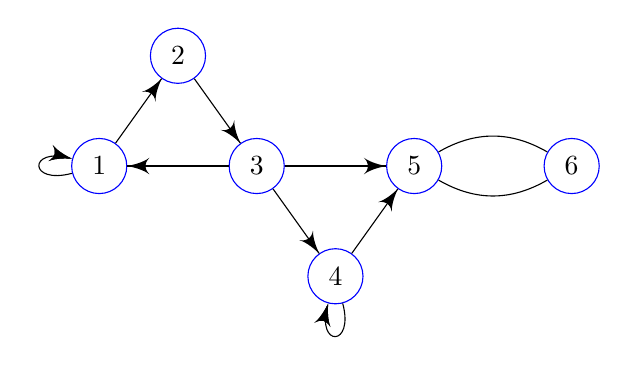
\begin{tikzpicture}
      \node [mstate] (1) at (0, 0) {$1$};
      \node [mstate] (2) at (1, 1.4) {$2$};
      \node [mstate] (3) at (2, 0) {$3$};
      \node [mstate] (4) at (3, -1.4) {$4$};
      \node [mstate] (5) at (4, 0) {$5$};
      \node [mstate] (6) at (6, 0) {$6$};
      \draw (1) edge [loop left, ->] (1);
      \draw (1) edge [->] (2);
      \draw (2) edge [->] (3);
      \draw (3) edge [->] (1);
      \draw (3) edge [->] (4);
      \draw (3) edge [->] (5);
      \draw (4) edge [->] (5);
      \draw (4) edge [loop below, ->] (4);
      \draw (5) edge [bend left, ->] (6);
      \draw (6) edge [bend left, ->] (5);
    \end{tikzpicture}
  \end{center}
  We see that the communicating classes are $\{1, 2, 3\}$, $\{4\}$, $\{5, 6\}$, where $\{5, 6\}$ is closed.
\end{eg}

\section{Recurrence or transience}
We adopt the following notation:
\[
  \P_i(A) = \P(A| X_0 = i),
\]
and
\[
  \E_i(Z) = \E(Z| X_0 = i).
\]
Suppose we start from $i$, and randomly wander around. Eventually, we may or may not get to $j$. If we do, there is a time at which we first reach $j$. We call this the \emph{first passage time}, written
\[
  T_j = \min\{n \geq 1: X_n = j\}.
\]
Note that we require $n \geq 1$. Otherwise $T_i$ would always be $0$.

The \emph{first passage probability} is
\[
  f_{ij}(n) = \P_i(T_j = n).
\]
\begin{defi}[Recurrent state]
  A state $i\in S$ is \emph{recurrent} (or \emph{persistent}) if
  \[
    \P_i (T_i < \infty) = 1,
  \]
  ie. we will eventually get back to the space. Otherwise, we call the state \emph{transient}.
\end{defi}
Note that transient does \emph{not} mean we don't get back. It's just that we are not sure that we will get back. We can (but will not) show that if a state is recurrent, then the probability that we return to $i$ infinitely many times is also $1$.

Note that when we discuss about recurrent and transient states, we are often concerned with an infinite state space. In the infinite state space, a state is transient because we are likely to wander to a place far far away and not get back. However, in a finite state space, transience happens only if we are stuck somewhere, ie. we are not in an irreducible state space. This is not too interesting.

Our current objective is to show the following:
\begin{thm}
  $i$ is recurrent iff $\sum_n p_{ii}(n) = \infty$.
\end{thm}
The technique to prove this would be to use generating functions. We need to first decide what sequence to work with. For any fixed $i, j$, consider the sequence $p_{ij}(n)$ as a sequence in $n$. Then we define
\[
  P_{ij}(s) = \sum_{n = 0}^\infty p_{ij}(n) s^n.
\]
We also define
\[
  F_{ij}(S) = \sum_{n = 0}^\infty f_{ij}(n) s^n,
\]
where $f_{ij}$ is our first-pass probability. For the sake of clarity, we make it explicit that $p_{ij}(0) = \delta_{ij}$, and $f_{ij}(0) = 0$.

Our proof would be heavily based on the result below:
\begin{thm}[]
  \[
    P_{ij}(s) = \delta_{ij} + F_{ij}(s)P_{jj}(s),
  \]
  for $-1 < s \leq 1$.
\end{thm}

\begin{proof}
  Using the law of total probability
  \begin{align*}
    p_{ij}(n) &= \sum_{m = 1}^n \P_i(X_n = j| T_j = m) \P_i(T_j = m) \\
    \intertext{Using the Markov property, we can write this as}
    &= \sum_{m = 1}^n \P(X_n = j| X_m = j) \P_i(T_j = m)\\
    &= \sum_{m = 1}^n p_{jj}(n - m) f_{ij}(m).
  \end{align*}
  We can multiply through by $s^n$ and sum over all $n$ to obtain
  \[
    \sum_{n = 1}^\infty p_{ij}(n) S^n = \sum_{n = 1}^\infty \sum_{m = 1}^n p_{jj}(n - m)s^{n - m} f_{ij}(m)s^m.
  \]
  The left hand side is \emph{almost} the generating function $P_{ij}(s)$, except that we are missing an $n = 0$ term, which is $p_{ij}(0) = \delta_{ij}$. The right hand side is the ``convolution'' of the power series $P_{jj}(s)$ and $F_{ij}(s)$, which we can write as the product $P_{jj}(s) F_{ij}(s)$. So
  \[
    P_{ij}(s) - \delta_{ij} = P_{ij}(s) F_{ij}(s).
  \]
\end{proof}

Before we actually prove our theorem, we need one helpful result from Analysis that allows us to deal with power series nicely.
\begin{lemma}[Abel's lemma]
  Let $u_1, u_2, \cdots$ be real numbers such that $U(s) = \sum_{n} u_n s^n$ converges for $0 < s < 1$. Then
  \[
    \lim_{s\to 1^-} U(s) = \sum_n u_n.
  \]
\end{lemma}
Proof is an exercise for Analysis.

We now prove the theorem we initially wanted to show
\begin{thm}
  $i$ is recurrent iff $\sum_n p_{ii}(n) = \infty$.
\end{thm}

\begin{proof}
  Using $j = i$ in the above formula, for $0 < s < 1$, we have
  \[
    P_{ii}(s) = \frac{1}{1 - F_{ii} (s)}.
  \]
  Here we need to be careful that we are not dividing by $0$. Thiw would be a problem if $F_{ii}(s) = 1$. By definition, we have
  \[
    F_{ii}(s) = \sum_{n = 1}^\infty f_{ii}(n) s^n.
  \]
  Also, by definition of $f_{ii}$, we have
  \[
    F_{ii}(1) = \sum_n f_{ij}(n) = \P(\text{ever returning to }1) \leq 1.
  \]
  So for $|s| < 1$, $F_{ii}(s) < 1$. So we are not dividing by zero. Now we use our original equation
  \[
    P_{ii}(s) = \frac{1}{1 - F_{ii} (s)},
  \]
  and take the limit as $s \to 1$. By Abel's lemma, we know that the left hand side is
  \[
    \lim_{s \to 1}P_{ii}(s) = P_{ii}(1) = \sum_n p_{ii}(n).
  \]
  The other side is
  \[
    \lim_{s \to 1}\frac{1}{1 - F_{ii}(s)} = \frac{1}{1 - \sum f_{ii}(n)}.
  \]
  Hence we have
  \[
    \sum_n p_{ii}(n) = \frac{1}{1 - \sum f_{ii}(n)}.
  \]
  Since $\sum f_{ii}(n)$ is the probability of ever returning, the probability of ever returning is 1 if and only if $\sum_n p_{ii}(n) = \infty$.
\end{proof}

Using this result, we can check if a state is recurrent. However, a Markov chain has many states, and it would be tedious to check if every state is recurring. Thus we have the following helpful result.
\begin{thm}[]
  Let $C$ be a communicating class. Then
  \begin{enumerate}
    \item Either every state in $C$ is recurrent, or every state is transient.
    \item If $C$ contains a recurrent state, then $C$ is closed.
  \end{enumerate}
\end{thm}

\begin{proof}\leavevmode
  \begin{enumerate}
    \item Let $i \leftrightarrow j$ and $i \not =j$. Then by definition of communicating, there is some $m$ such that $p_{ij}(m) = \alpha > 0$, and some $n$ such that $p_{ji}(n) = \beta > 0$. So for each $k$, we have
      \[
        p_{ii}(m + k + n) \geq p_{ij}(m) p_{jj}(k) p_{ji}(n) = \alpha\beta p_{jj}(k).
      \]
      So if $\sum_k p_{jj}(k) = \infty$, then $\sum_r p_{ii}(r) = \infty$. So $j$ recurrent implies $i$ recurrent. Similarly, $i$ recurrent implies $j$ recurrent.
    \item If $C$ is not closed, then there is a non-zero probability that we leave the class and never get back. So the states are not recurrent.
  \end{enumerate}
\end{proof}

Note that there is a profound difference between a finite state space and an infinite state space. A finite state space can be represented by a finite matrix, and we are all very familiar with a finite matrices. We can use everything we know about finite matrices from IA Vectors and Matrices. However, infinite matrices are weirder.

For example, any finite transition matrix $P$ has an eigenvalue of $1$. This is since the row sums of a transition matrix is always $1$. So if we multiply $P$ by $\mathbf{e} = (1, 1, \cdots, 1)$, then we get $\mathbf{e}$ again. However, this is not true for infinite matrices, since we usually don't usually allow arbitrary infinite vectors. We usually restrict our focus to vectors $\mathbf{x}$ such that $\sum x_i^2$ is finite. In this case the vector $\mathbf{e}$ is not allowed, and the transition matrix need not have eigenvalue $1$.

Another thing about a finite state space is that probability ``cannot escape''. We can think of a Markov chain as a flow of probabilities around the state space, with the probability distribution moving around in every step. If we have a finite state space, all the probability must be contained within your finite state space. However, if we have an infinite state space, then probabilities can just drift away to infinity.

In particular, we have the following result:
\begin{thm}[]
  In a finite state space,
  \begin{enumerate}
    \item There exists at least one recurrent state.
    \item If the chain is irreducible, every state is recurrent.
  \end{enumerate}
\end{thm}

\begin{proof}
  Recall that
  \[
    P_{ij}(s) = \delta_{ij} + P_{jj}(s) F_{ij}(s).
  \]
  If $j$ is transient, then $\sum_n p_{jj}(n) = P_{jj}(1) < \infty$. Hence $P_{ij}(1) < \infty$. By Abel's lemma, $P_{ij}(1)$ is given by
  \[
    P_{ij}(1) = \sum_n p_{ij}(n).
  \]
  Since this is finite,  we must have $p_{ij}\to 0$.

  Since we know that
  \[
    \sum_{j\in S}p_{ij}(n) = 1,
  \]
  If every state is transient, then for all $j$, $\sum p_{ij}(n) \to 0$ as $n\to \infty$. This is a contradiction.
\end{proof}

\begin{thm}[P\'olya's theorem]
  Consider $\Z^d = \{(x_1, x_2, \cdots, x_d): x_i \in \Z\}$. This generates a graph with $x\sim y$ if $|x - y| = 1$, where $|\ph |$ is the Euclidean norm.
  \begin{center}
    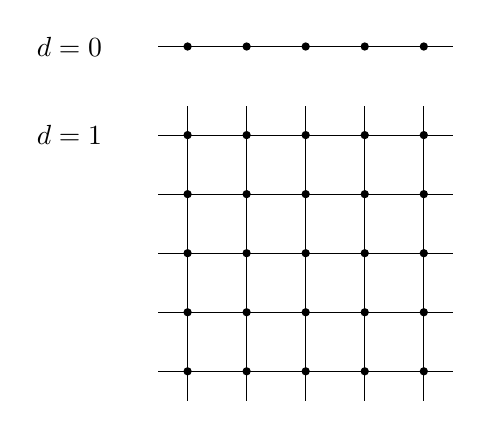
\begin{tikzpicture}[scale=0.75]
      \node at (-4, 0) {$d = 0$};
      \draw (-2.5, 0) -- (2.5, 0);
      \foreach \x in {-2,-1,...,2} {
        \node [circ] at (\x, 0) {};
      }
      \begin{scope}[shift={(0, -3.5)}]
        \node at (-4, 2) {$d = 1$};
        \foreach \x in {-2, -1,...,2} {
          \foreach \y in {-2,-1,...,2} {
            \node [circ] at (\x, \y) {};
          }
        }
        \foreach \x in {-2, -1,...,2} {
          \draw (\x, -2.5) -- (\x, 2.5);
          \draw (-2.5, \x) -- (2.5, \x);
        }
      \end{scope}
    \end{tikzpicture}
  \end{center}
  Consider a random walk in $\Z^d$. At each step, it moves to a neighbour, each chosen with equal probability, ie.
   \[
    \P(X_{n + 1} = j| X_n = i) =
    \begin{cases}
      \frac{1}{2d} & |j - i| = 1\\
      0 & \text{otherwise}
    \end{cases}
  \]
  This is an irreducible chain, since it is possible to get from one point to any other point. So the points are either all recurrent or all transient.

  The theorem says this is recurrent iff $d = 1$ or $2$.
\end{thm}
Intuitively, this makes sense since if we have more dimensions, then it is easier to get lost.

\begin{proof}
  We will start with the case $d = 1$. We want to show that $\sum p_{0, 0}(n) = \infty$. Then we know the origin is recurrent. However, we can simplify this a bit. It is impossible to get back to the origin in an odd number of steps. So we can instead write $\sum p_{0, 0}(2n)$. However, we can write down this expression immediately. To return to the origin after $2n$ steps, we need to have made $n$ steps to the left, and $n$ steps to the right, in any order. So we have
  \[
    p_{0, 0}(2n) = \P(n\text{ steps left}, n\text{ steps right}) = \binom{2n}{n} \left(\frac{1}{2}\right)^{2n}.
  \]
  To show if this converges, it is not helpful to work with these binomial coefficients and factorials. So we use Stirling's formula $n! \simeq \sqrt{2\pi n}\left(\frac{n}{e}\right)^n$. If we plug this in, we get
  \[
    p_{0, 0}(2n) \sim \frac{1}{\sqrt{\pi n}}.
  \]
  This tends to $0$, but really slowly, and even more slowly than the harmonic series. So we have $\sum p_{0, 0}(2n) = \infty$.

  In the $d = 2$ case, suppose after $2n$ steps, I have taken $r$ steps right, $\ell$ steps left, $u$ steps up and $d$ steps down. We must have $r + \ell + u + d = 2n$, and we need $r = \ell, u = d$ to return the origin. So we let $r = \ell = m, u = d = n - m$. So we get
  \begin{align*}
    p_{0, 0}(2n) &= \left(\frac{1}{4}\right)^{2n} \sum_{m = 0}^n \binom{2n}{m, m, n - m, n - m} \\
    &= \left(\frac{1}{4}\right)^{2n} \sum_{m = 0}^n \frac{(2n)!}{(m!)^2 ((n - m)!)^2} \\
    &= \left(\frac{1}{4}\right)^{2n} \binom{2n}{n}\sum_m \left(\frac{n!}{m!(n - m)!}\right)^2\\
    &= \left(\frac{1}{4}\right)^{2n} \binom{2n}{n}\sum_m \left(\binom{n}{m}\binom{n}{n - m}\right)^2\\
    \intertext{We now use a well-known identity (proved in IA Numbers and Sets) to obtain}
    &= \left(\frac{1}{4}\right)^{2n} \binom{2n}{n} \binom{2n}{n}\\
    &= \left[\binom{2n}{n} \left(\frac{1}{2}\right)^{2n}\right]^2\\
    &\sim \frac{1}{\pi n}.
  \end{align*}
  So the sum diverges. So this is recurrent. Note that the two-dimensional probability turns out to be the square of the one-dimensional probability. Is this a coincidence? Or is there a reason why? Does this extend to higher dimensions? We would be able to explain why this happens, but it unfortunately does not extend straightforwardly to higher dimensions.

  In the $d = 3$ case, we have
  \[
    p_{0, 0}(2n) = \left(\frac{1}{6}\right)^{2n}\sum_{i + j + k = n}\frac{(2n)!}{(i!j!k!)^2}.
  \]
  This time, there is no neat combinatorial formula. Since we want to show this is summable, we can try to bound this from above. We have
  \begin{align*}
    p_{0, 0}(2m) &= \left(\frac{1}{6}\right)^{2n} \binom{2n}{n} \sum \left(\frac{n!}{i!j!k!}\right)^2\\
    &= \left(\frac{1}{2}\right)^{2n} \binom{2n}{n} \sum \left(\frac{n!}{3^n i!j!k!}\right)^2\\
    \intertext{Why do we write it like this? We are going to use the identity $\displaystyle \sum_{i + j + k = n} \frac{n!}{3^n i!j!k!} = 1$. Where does this come from? Suppose we have three urns, and throw $n$ balls into it. Then the probability of getting $i$ balls in the first, $j$ in the second and $k$ in the third is exactly $\frac{n!}{3^n i!j!k!}$. Summing over all possible combinations of $i$, $j$ and $k$ gives the total probability of getting in any configuration, which is $1$. So we can bound this by}
    &\leq \left(\frac{1}{2}\right)^{2n}\binom{2n}{n} \max\left(\frac{n!}{3^n i!j!k!}\right)\sum \frac{n!}{3^n i!j!k!}\\
    &= \left(\frac{1}{2}\right)^{2n}\binom{2n}{n} \max\left(\frac{n!}{3^n i!j!k!}\right)
    \intertext{To find the maximum, we can replace the factorial by the gamma function and use Lagrange multiplier. However, we would just argue that the maximum can be achieved when $i$, $j$ and $k$ are as close to each other as possible. So we get}
    &\leq \left(\frac{1}{2}\right)^{2n}\binom{2n}{n} \frac{n!}{3^n}\left(\frac{1}{\lfloor n/3\rfloor!}\right)^3\\
    &\leq Cn^{-3/2}
  \end{align*}
  for some constant $C$ using Stirling's formula. So $\sum p_{0,0}(2n) < \infty$ and the chain is transient. We can prove similarly for higher dimensions.
\end{proof}

Let's get back to why the two dimensional probability is the square of the one-dimensional probability. This square might remind us of independence. However, it is obviously not true that horizontal movement and vertical movement are independent --- if we go sideways in one step, then we cannot move vertically. So we need something more sophisticated.

We write $X_n = (A_n, B_n)$. What we do is that we try to rotate our space. We are going to record our coordinates in a pair of axis that is rotated by $45^\circ$.
\begin{center}
  \begin{tikzpicture}
    \draw [->] (-2, 0) -- (4, 0) node [right] {$A$};
    \draw [->] (0, -3) -- (0, 3) node [above] {$B$};

    \node [circ] at (3, 2) {};
    \node [right] at (3, 2) {$(A_n, B_n)$};

    \draw [mred, ->] (-1, -1) -- (3, 3) node [anchor = south west] {$V$};
    \draw [mred, ->] (-1, 1) -- (3, -3) node [anchor = north west] {$U$};

    \draw [mred, dashed] (3, 2) -- (0.5, -0.5) node [anchor = north east] {$U_n/\sqrt{2}$};
    \draw [mred, dashed] (3, 2) -- (2.5, 2.5) node [anchor = south east] {$V_n/\sqrt{2}$};
  \end{tikzpicture}
\end{center}
We can define the new coordinates as
\begin{align*}
  U_n &= A_n - B_n\\
  V_n &= A_n + B_n
\end{align*}
In each step, either $A_n$ or $B_n$ change by one step. So $U_n$ and $V_n$ \emph{both} change by $1$. Moreover, they are independent. So we have
\begin{align*}
  p_{0, 0}(2n) &= \P(A_n = B_n = 0)\\
  &= \P(U_n = V_n = 0)\\
  &= \P(U_n = 0)\P (V_n = 0)\\
  &= \left[\binom{2n}{n}\left(\frac{1}{2}\right)^{2n}\right]^2.
\end{align*}
\subsection{Hitting probabilities}
In general, we might have a Markov chain, and there are some states we want to reach, or don't want to reach. For example, we might be in a casino, and we want to win, say, a million, and don't want to go bankrupt. So we want to study how likely and when we will reach these states.

In general, let $A \subseteq S$.
\begin{defi}[Hitting time]
  The \emph{hitting time} of $A \subseteq S$ is the random variable $H^A = \min\{n \geq 0: X_n \in A\}$. In particular, if we start in $A$, then $H^A = 0$. We also have
  \[
    h_i^A = \P_i(H^A < \infty) = \P_i(\text{ever reach }A).
  \]
\end{defi}

We are going to have an important result about the hitting time:
\begin{thm}
  The vector $(h_i^A: i \in S)$ satisfies
  \[
    h_i^A =
    \begin{cases}
      1 & i \in A\\
      \sum_{j \in S}p_{ij}h_j^A & i \not \in A
    \end{cases},
  \]
  and is \emph{minimal} in that for any non-negative solution $(x_i: i \in S)$ to these equations, we have $h_i^a \leq x_i$ for all $i$.
\end{thm}
The first part is easy to show using the definition, but it takes some more work to show that the real $h_i^A$ is minimal. The proof, however, is almost the same as that for random walks in IA Probability.

\begin{proof}
  By definition, $h_i^A = 1$ if $i \in A$. Then we have
  \[
    h_i^A = \P_i(H^A < \infty) = \sum_{j\in S} \P_i(H^A < \infty | X_1 = j)p_{ij} = \sum_{j\in S}h_{j}^A p_{ij}.
  \]
  So $h_i^A$ is a solution.

  To show that $h_i^A$ is the minimal solution, suppose $x = (x_i: i \in S)$ is a non-negative solution, ie.
  \[
    x_i^A =
    \begin{cases}
      1 & i \in A\\
      \sum_{j \in S}p_{ij}x_j^A & i \not \in A
    \end{cases},
  \]
  If $i \in A$, we have $h_i^A = x_i = 1$. Otherwise, we can write
  \begin{align*}
    x_i &= \sum_j p_{ij}x_j \\
    &= \sum_{j \in A}p_{ij}x_j + \sum_{j \not\in A}p_{ij}x_j \\
    &= \sum_{j \in A}p_{ij} + \sum_{j \not\in A}p_{ij}x_j \\
    &\geq \sum_{j \in A}p_{ij}\\
    &= \P_i(H^A = 1).
  \end{align*}
  By iterating this process, we can write
  \begin{align*}
    x_i &= \sum_{j \in A} p_{ij} + \sum_{j \not\in A} p_{ij}\left(\sum_k p_{ik} x_k\right) \\
    &= \sum_{j \in A} p_{ij} + \sum_{j \not\in A} p_{ij}\left(\sum_{k\in A} p_{ik} x_k + \sum_{k \not\in A} p_{ik}x_k\right)\\
    &\geq \P_i (H^A = 1) + \sum_{j \not \in A, k \in A}p_{ij}p_{jk}\\
    &= \P_i(H^A = 1) + \P_i(H^A = 2)\\
    &= \P_i (H^A \leq 2).
  \end{align*}
  By induction, we obtain
  \[
    x_i \geq \P_i(H^A \leq n)
  \]
  for all $n$. Taking the limit as $n \to \infty$, we get
  \[
    x_n \geq \P_i(H^A \leq \infty) = h_i^A.
  \]
\end{proof}
The next question we want to ask is how long it will take for us to hit $A$. We want to find $\E_i(H^A) = k_i^A$. Note that we have to be careful --- if there is a chance that we never hit $A$, then it is $H^A$ could be infinite, and $\E_i(H^A) = \infty$. This occurs if $h_i^A < 1$. So often we are only interested in the case where $h_i^A < 1$.

Nevertheless, we have the following result:
\begin{thm}[]
  $(k_i^A: i \in S)$ is the minimal non-negative solution to
  \[
    k_i^A =
    \begin{cases}
      0 & i \in A\\
      1 + \sum_j p_{ik}k_j^A & i \not\in A.
    \end{cases}
  \]
\end{thm}
Note that we have this ``$1 +$'' since when we move from $i$ to $j$, one step has already passed.

The proof is almost the same as the proof we had above.
\begin{proof}
  The proof that $(k_i^A)$ satisfies the equations is the same as before.

  Now let $(y_i : i\in S)$ be a non-negative solution. We show that $y_i \geq k_i^A$.

  If $i \in A$, we get $y_i = k_i^A = 0$. Otherwise, suppose $i\not\in A$. Then we have
  \begin{align*}
    y_i &= 1 + \sum_j p_{ij}y_j\\
    &= 1 + \sum_{j \in A}p_{ij}y_j + \sum_{j\not\in A}p_{ij}y_j\\
    &= 1 + \sum_{j\not\in A}p_{ij}y_j\\
    &= 1 + \sum_{j \not\in A}p_{ij}\left(1 + \sum_{k\not\in A} p_{jk}y_k\right)\\
    &\geq 1 + \sum_{j \not\in A} p_{ij}\\
    &= \P_i(H^A \geq 1) + \P_i(H^A \geq 2).
  \end{align*}
  By induction, we know that
  \[
    y_i \geq \P_i (H^A \geq 1) + \cdots + \P_i(H^A \geq n)
  \]
  for all $n$. Let $ n\to \infty$. Then we get
  \[
    y_i \geq \sum_{m \geq 1}\P_i(H^A \geq m) = \sum_{m \geq 1} m\P_i(H^a = m)= k_i^A.
  \]
\end{proof}

\begin{eg}[Gambler's ruin]
  This time, we will consider a random walk on $\N$. In each step, we either move to the right with probability $p$, or to the left with probability $q = 1 - p$. What is the probability of every hitting $0$ from a given initial point? In other words, we want to find $h_i = h_i^{\{0\}}$.

  We know $h_i$ is the minimal solution to
  \[
    h_i =
    \begin{cases}
      1 & i = 0\\
      qh_{i - 1} + ph_{i + 1} & i \not= 0.
    \end{cases}
  \]
  What are the solutions to these equations? We can view this as a difference equation
  \[
    ph_{i + 1} - h_i + qh_{i - 1} = 0,\quad i \geq 1.
  \]
  with the boundary condition that $h_0 = 1$. We all know how to solve difference equations, so let's just jump to the solution.

  If $p \not= q$, ie. $p \not= \frac{1}{2}$, then the solution has the form
  \[
    h_i = A + B\left(\frac{q}{p}\right)^i
  \]
  for $i \geq 0$. If $p < q$, then for large $i$, $\left(\frac{q}{p}\right)^i$ is very large and blows up. However, since $h_i$ is a probability, it can never blow up. So we must have $B = 0$. So $h_i$ is constant. Since $h_0 = 1$, we have $h_i = 1$ for all $i$. So we always get to $0$.

  If $p > q$, since $h_0 = 1$, we have $A + B = 1$. So
  \[
    h_i = \left(\frac{q}{p}\right)^i + A\left(1 - \left(\frac{q}{p}\right)^i\right).
  \]
  This is in fact a solution for all $A$. So we want to find the smallest solution.

  As $i \to\infty$, we get $h_i \to A$. Since $h_i \geq 0$, we know that $A \geq 0$. Subject to this constraint, the minimum is attained when $A = 0$ (since $(q/p)^i$ and $(1 - (q/p)^i)$ are both positive).

  There is another way to solve this. We can give ourselves a ceiling, ie. we also stop when we hit $k > 0$, ie. $h_k = 1$. We now have two boundary conditions and can find a unique solution. Then we take the limit as $k \to \infty$. This is the approach taken in IA Probability.

  Here if $p = q$, then by the same arguments, we get $h_i = 1$ for all $i$.
\end{eg}

\begin{eg}[Birth-death chain]
  Let $(p_i: i \geq 1)$ such that $p_i \in (0, 1)$. We let $q_i = 1 - p_i$. We let $\N$ be our state space and define the transition probabilities to be
  \[
    p_{i, i + 1} = p_i,\quad p_{i, i - 1} = q_i.
  \]
  This is a more general case of the random walk --- in the random walk we have a constant $p_i$ sequence.

  This is a general model for population growth, for the change in population depends on what the current population is. Here each ``step'' does not correspond to some unit time, since births and deaths occur rather randomly. Instead, we just make a ``step'' whenever some birth or death occurs, regardless of what time they occur.

  Here, if we have no people left, then it is impossible for us to reproduce and get more population. So we have
  \[
    p_{0, 0} = 1.
  \]
  We say $0$ is \emph{absorbing} in that $\{0\}$ is closed. We let $h_i = h_i^{\{0\}}$. We know that
  \[
    h_0 = 1,\quad p_i h_{i + 1} - h_i + q_i h_{i - 1} = 0,\quad i \geq 1.
  \]
  This is no longer a difference equation, since the coefficients depends on the index $i$. To solve this, we rewrite this as
  \[
    p_i h_{i + 1} - h_i + q_i h_{i - 1} = p_i h_{i + 1} - (p_i + q_i) h_i + q_i h_{i - 1}.
  \]
  We let $u_i = h_{i - 1} - h_i$. Then our equation becomes
  \[
    u_{i + 1} = \frac{q_i}{p_i} u_i.
  \]
  We can iterate this to become
  \[
    u_{i + 1} = \left(\frac{q_i}{p_i}\right)\left(\frac{q_{i - 1}}{p_{i - 1}}\right) \cdots \left(\frac{q_1}{p_1}\right) u_1.
  \]
  We let
  \[
    \gamma_i = \frac{q_1q_2\cdots q_i}{p_1p_2\cdots p_i}.
  \]
  Then we get $u_{i + 1} = \gamma_i u_1$. Now we want to retrieve our $h_i$. We can do this by summing the equation $u_i = h_{i - 1} - h_i$. So we get
  \[
    h_0 - h_i = u_1 + u_2 + \cdots + u_i.
  \]
  Using the fact that $h_0 = 1$, we get
  \[
    h_i = 1 - u_1(\gamma_0 + \gamma_1 + \cdots + \gamma_{i - 1}),
  \]
  where $\gamma_0 = 1$. Here we have a parameter $u_1$, and we need to find out what this is. Our theorem tells us the value of $u_1$ minimizes $h_i$. This all depends on the value of
  \[
    S = \sum_{i = 0}^\infty \gamma_i.
  \]
  By the law of excluded middle, $S$ either diverges or converges. If $S = \infty$, then we must have $u_1 = 0$. Otherwise, $h_i$ blows up for large $i$, but we know that $0 \leq h_i \leq 1$. If $S$ is finite, then $u_1$ can be non-zero. We know that the $\gamma_i$ are all positive. So to minimize $h_i$, we need to maximize $u_1$. We cannot make $u_1$ arbitrarily large, since this will make $h_i$ negative. Taking the limit as $i \to\infty$, we know that the maximum value of $u_1$ satisfies
  \[
    0 = 1 - u_1 S.
  \]
  In other words, $u_1 = 1/S$. Then we have
  \[
    h_i = \frac{\sum_{k = i}^\infty \gamma_k}{\sum_{k = 0}^\infty \gamma_k}.
  \]
\end{eg}

\subsection{Stopping times and strong Markov property}
We are going to state the \emph{strong} Markov property and see applications of it. Before this, we should know what the \emph{weak} Markov property is. We have, in fact, already seen the weak Markov property. It's just that we called it the ``Markov property' instead.

In probability, we often have ``strong'' and ``weak'' versions of things. For example, we have the strong and weak law of large numbers. In general, the difference is that the weak versions are expressed in terms of probabilities, while the strong versions are expressed in terms of random variables. Initially, when people first started developing probability theory, they just talked about probability distributions like the Poisson distribution or the normal distribution. However, later it turned out it is often nicer to talk about random variables instead. After messing with random variables, we can just take expectations or evaluate probabilities to get the corresponding statement about probability distributions. Hence usually the ``strong'' versions imply the ``weak'' version, but not the other way round.

In this case, recall that we defined the Markov property in terms of the probabilities at some fixed time. We have some fixed time $t$, and we want to know the probabilities of events after $t$ in terms of what happened before $t$. In the strong Markov property, we will allow $t$ to be a random variable, and say something slightly more involved. However, we will not allow $T$ to be any random variable, but just some nice ones.

\begin{defi}[Stopping time]
  Let $X$ be a Markov chain. A random variable $T$ (which is a function $\Omega \to \N\cup \{\infty\}$) is a \emph{stopping time} for the chain $X = (X_n)$ if for $n \geq 0$, the event $\{T = n\}$ is given in terms of $X_0, \cdots, X_1, X_n$.
\end{defi}
For example, suppose we are in a casino and gambling. We let $X_n$ be the amount of money we have at time $n$. Then we can set our stopping time as ``the time when we have $\$10$ left''. This is a stopping time, in the sense that we can use this as a guide to when to stop --- it is certainly possible to set yourself a guide that you should leave the casino when you have $\$10$ left. However, it does not make sense to say ``I will leave if the next game will make me bankrupt'', since there is no way to tell if the next game will make you bankrupt (it certainly will not if you win the game!). Hence this is not a stopping time.

\begin{eg}
  The hitting time $H^A$ is a stopping time. This is since $\{H^A = n\} = \{X_i \not\in A\text{ for }i < n\}  \cap \{X_n \in A\}$. We also know that $H^A + 1$ is a stopping time since it only depends in $X_i$ for $i \leq n - 1$. However, $H^A - 1$ is not a stopping time since it depends on $X_{n + 1}$.
\end{eg}

We can now state the strong Markov property, which is expressed in a rather complicated manner but can be useful at times.
\begin{thm}[Strong Markov property]
  Let $X$ be a Markov change with transition matrix $P$, and let $T$ be a stopping time for $X$. Given $T < \infty$ and $X_T = i$, the chain $(X_{T + k}: k \geq 0)$ is a Markov chain with transition matrix $P$ with initial distribution $X_{T + 0} = i$, and this Markov chain is independent of $X_0, \cdots, X_T$.
\end{thm}
Proof is omitted.

\begin{eg}[Gambler's ruin]
  Again, this is the Markov chain taking values on the non-negative integers, moving to the right with probability $p$ and left with probability $q = 1 - p$. $0$ is an absorbing state, since we cannot escape zero.

  Instead of computing the probability of hitting zero, we want to find the time it takes to get to $0$, ie.
  \[
    H = \inf\{n \geq 0: X_n = 0\}.
  \]
  Note that the infimum of the empty set is $+\infty$, ie. if we never hit zero, we say it takes infinite time. What is the distribution of $H$? We define the generating function
  \[
    G_i(s) = \E_i(s^H) = \sum_{n = 0}^\infty s^n \P_i(H = n),\quad |s| < 1.
  \]
  Note that we need the requirement that $|s| < 1$, since it is possible that $H$ is infinite, and we would not want to think whether the sum converges when $s = 1$. However, we know that it does for $|s| < 1$.

  We have
  \[
    G_1(s) = \E_1(s^H) = p\E_1(s^H|X_1 = 2) + q\E_1(s^H|X_1 = 0).
  \]
  How can we simplify this? The second term is easy, since if $X_1 = 0$, then we must have $H = 1$. So $\E_1(s^H|X_1 = 0) = s$. The second term is more tricky. We are now at $2$. To get to $0$, we need to pass through $1$. So the time needed to get to $0$ is the time to get from $2$ to $1$ (say $H'$), plus the time to get from $1$ to $0$ (say $H''$). We know that $H'$ and $H''$ have the same distribution as $H$, and by the strong Markov property, they are independent. So
  \[
    G_1 = p\E_1(s^{H' + H'' + 1}) + qs = psG_1^2 + qs.
  \]
  Solving this, we get two solutions
  \[
    G_1 (s) = \frac{1 \pm \sqrt{1 - 4pqs^2}}{2ps}.\tag{$*$}
  \]
  We have to be careful here. This result says that for each value of $s$, $G_1(s)$ is \emph{either} $\frac{1 + \sqrt{1 - 4pqs^2}}{2ps}$ \emph{or} $\frac{1 - \sqrt{1 - 4pqs^2}}{2ps}$. It does \emph{not} say that there is some consistent choice of $+$ or $-$ that works for everything.

  However, we know that if we suddenly change the sign, then $G_1(s)$ will be discontinuous at that point, but $G_1$, being a power series, has to be continuous. So the solution must be either $+$ for all $s$, or $-$ for all $s$.

  To determine the sign, we can look at what happens when $s = 0$. We see that the numerator becomes $1 \pm 1$, while the denominator is $0$. We know that $G$ converges at $s = 0$. Hence the numerator must be $0$. So we must pick $-$, ie.
  \[
    G_1 (s) = \frac{1 - \sqrt{1 - 4pqs^2}}{2ps}.
  \]
  We can find $\P_1(H = k)$ by expanding the Taylor series.

  What is the probability of ever hitting $0$? This is
  \[
    \P_1(H < \infty) = \sum_{n = 1}^\infty \P(H = n) = \lim_{s\to 1} G_1(s) = \frac{1 - \sqrt{1 - 4pq}}{2p}.
  \]
  We can rewrite this using the fact that $q = 1 - p$. So $1 - 4pq = 1 - 4p(1 - p) = (1 - 2p)^2 = |q - p|^2$. So we can write
  \[
    \P_1(H < \infty) = \frac{1 - |p - q|}{2p} =
    \begin{cases}
      1 & p \leq q\\
      \frac{q}{p} & p > q
    \end{cases}
  \]
  Using this, we can also find $\mu = \E_1(H)$. Firstly, if $p > q$, then it is possible that $H = \infty$. So $\mu = \infty$. If $p \leq q$, we can find $\mu$ by differentiating $G_1(s)$ and evaluating at $s = 1$. Doing this directly would result it horrible and messy algebra, which we want to avoid. Instead, we can differentiate $(*)$ and obtain
  \[
    G_1' = pG_1^2 + ps 2 G_1G_1' + q.
  \]
  We can rewrite this as
  \[
    G_1'(s) = \frac{pG(s)^2 + q}{1 - 2ps G(s)}.
  \]
  By Abel's lemma, we have
  \[
    \mu = \lim_{s \to 1}G'(s) =
    \begin{cases}
      \infty & p = \frac{1}{2}\\
      \frac{1}{p - q} & p < \frac{1}{2}.
    \end{cases}
  \]
\end{eg}
\section{Classification of states}
So far, we have classified chains in say, irreducible and reducible chains. We have also seen that states can be recurrent or transience. By definition, a state is recurrent if the probability of returning to it is infinite. However, we can further classify recurrent states. Even if a state is recurrent, it is possible that the expected time of returning is infinite. So it is likely that we return to the original state only after a very long time. On the other hand, it might be that are very likely to return quickly, and the expected time of returning is finite. It turns out this distinction can affect the long-term behaviour of the chain.

First we have the following proposition, which tells us that if a state is recurrent, then we are expected to return to it infinitely many times.
\begin{thm}
  Suppose $X_0 = i$. Let $V_i = |\{n \geq 1: X_n = i\}|$. Let $f_{ii} = \P_i(T_i < \infty)$. Then
  \[
    \P_i (V_i = r) = f_{ii}^r (1 - f_{ii}),
  \]
  since we have to return $r$ times, each with probability $f_{ii}$, and then never return.

  Hence, if $f_{ii} = 1$, then $\P_i(V_i = r) = 0$ for all $r$. So $\P_i(V_i = \infty) = 1$. Otherwise, $\P_i(V_i = r)$ is a genuine geometric distribution, and we get $\P_i(V_i < \infty) = 1$.
\end{thm}

\begin{proof}
  Exercise, using the strong Markov property.
\end{proof}

\begin{defi}[Mean recurrence time]
  Let $T_i$ be the returning time to a state $i$. Then the \emph{mean recurrence time} of $i$ is
  \[
    \mu_i = \E_i(T_i) =
    \begin{cases}
      \infty & i\text{ transient}\\
      \sum_{n = 1}^\infty n f_{ii}(n) & i\text{ recurrent}
    \end{cases}
  \]
\end{defi}

\begin{defi}[Null and positive state]
  If $i$ is recurrent, we call $i$ a \emph{null state} if $\mu_i = \infty$. Otherwise $i$ is \emph{non-null} or \emph{positive}.
\end{defi}

\begin{defi}[Period]
  The \emph{period} of a state $i$ is $d_i = \gcd\{n \geq 1: p_{ii}(n)> 0\}$.

  A state is \emph{aperiodic} if $d_i = 1$.
\end{defi}
For example, the period of $0$ in a simple random walk is $2$, since we can only return after an even number of steps.

\begin{defi}[Ergodic]
  A state $i$ is \emph{ergodic} if it is aperiodic and positive recurrent.
\end{defi}
These are the nice states.

Recall that recurrence is a class property --- if two states are in the same communicating class, then they are either both recurrent, or both transient. Is this true for the properties above as well? The answer is yes.

\begin{thm}[]
  If $i \leftrightarrow j$ are communicating, then
  \begin{enumerate}
    \item $d_i = d_j$.
    \item $i$ is recurrent iff $j$ is recurrent.
    \item $i$ is positive recurrent iff $j$ is positive recurrent.
    \item $i$ is ergodic iff $j$ is ergodic.
  \end{enumerate}
\end{thm}

\begin{proof}\leavevmode
  \begin{enumerate}
    \item Assume $i \leftrightarrow j$. Then there are $m, n \geq 1$ with $p_{ij}(m), p_{ji}(n) > 0$. By the Chapman-Kolmogorov inequality, we know that
      \[
        p_{ii}(m + r + n) \geq p_{ij}(m)p_{jj}(r)p_{ji}(n) \geq \alpha p_{jj}(r),
      \]
      where $\alpha = p_{ij}(m) p_{ji}(n) > 0$. Now let $D_j = \{r \geq 1: p_{jj}(r) > 0\}$. Then by definition, $d_j = \gcd D_j$.

      We have just shown that if $r \in D_j$, then we have $m + r + n \in D_i$. We also know that $n + m \in D_i$, since $p_{ii}(n + m) \geq p_{ij}(n)p_{ji}(m) > 0$. Then for any $r \in D_j$, we know that $d_i | m + r + n$, and also $d_i | m + n$. So $d_i | r$. Hence $\gcd D_i | \gcd D_j$. By symmetry, $\gcd D_i = \gcd D_j$.
    \item Proved before.
    \item This is deferred to a later time.
    \item Follows directly from (i), (ii) and (iii) by definition.
  \end{enumerate}
\end{proof}

We also have the following proposition we will use later one:
\begin{prop}
  If the chain is irreducible and $j \in S$ is recurrent, then
  \[
    \P(X_n = j\text{ for some }n \geq 1) = 1,
  \]
  regardless of the distribution of $X_0$.
\end{prop}
Note that this is not just the definition of recurrence, since recurrence says that if we start at $i$, then we will return to $i$. Here we are saying wherever we start, we will eventually visit $i$.

\begin{proof}
  Let
  \[
    f_{ij} = \P_i(X_n = j\text{ for some }n \geq 1).
  \]
  Since $j \to i$, there exists a \emph{least} integer $m \geq 1$ with $p_{ji}(m) > 0$. Since $m$ is least, we know that
  \[
    p_{ji}(m) = \P_j(X_m = i, X_r \not= j\text{ for }r < m).
  \]
  This is since we cannot visit $j$ in the path, or else we can truncate our path and get a shorter path from $j$ to $i$. Then
  \[
    p_{ji}(m)(1 - f_{ij}) \leq 1 - f_{jj}.
  \]
  This is since the left hand side is the probability that we first go from $j$ to $i$ in $m$ steps, and then never going from $i$ to $j$ again; while the right is the just probability of never returning to $j$ starting from $j$; and we know that it is easier to just not get back to $j$ than to go to $i$ in exactly $m$ steps and never returning to $j$. Hence if $f_{jj} = 1$, then $f_{ij} = 1$.

  Now let $\lambda_k = \P(X_j = k)$ be our initial distribution. Then
  \[
    \P(X_n = j\text{ for some }n \geq 1) = \sum_i \lambda_j \P_j (X_n =j\text{ for some }n \geq 1) = 1.
  \]
\end{proof}
\subsection{Invariant distributions}
We want to look at what happens in the long run. When we are dealing with real sequences $x_n$, we have a precise definition of what it means for $x_n \to x$. How can we define the convergence of a sequence of random variables $X_n$? These are not proper numbers, so we cannot just apply our usual definitions.

It turns out that the right way to think about convergence is to look at the probability mass function. For each $k \in S$, we ask if $\P(X_n = k)$ converges to anything.

In most cases, $\P(X_n = k)$ converges. Hence, this is not an interesting question to ask. What we would \emph{really} want to know is whether the limit is a probability mass function. It is, for example, possible that $\P(X_n = k) \to 0$ for all $k$, and the result is not a distribution.

Usually, when we want to prove that something converges, we first figure out what the limit should be, and then attempt to prove that convergence does indeed occur. In this case, recall that if we have a starting state $\lambda$, then the distribution of the $n$th step is given by $\lambda P^n$. We have the following trivial identity:
\[
  \lambda P^{n + 1} = (\lambda P^n) P.
\]
If the distribution converges, then we have $\lambda  P^n \to \pi$ for some $\pi$, and also $\lambda P^{n + 1} \to \pi$. Hence the limit $\pi$ satisfies
\[
  \pi P = \pi.
\]
We call these \emph{invariant distributions}.

\begin{defi}[Invariant distriubtion]
  Let $X_j$ be a Markov chain with transition probabilities $P$. The distribution $\pi = (\pi_k: k \in S)$ is an \emph{invariant distribution} if
  \begin{enumerate}
    \item $\pi_k \geq 0$, $\sum_k \pi_k = 1$.
    \item $\pi = \pi P$.
  \end{enumerate}
  The first condition just ensures that this is a genuine distribution.

  An invariant distribution is also known as an invariant measure, equilibrium distribution or steady-state distribution.
\end{defi}

\begin{thm}
  Consider an irreducible Markov chain. Then
  \begin{enumerate}
    \item There exists an invariant distribution if and only if some state is positive recurrent.
    \item If there is an invariant distribution $\pi$, then every state is positive recurrent, and
      \[
        \pi_i = \frac{1}{\mu_i}
      \]
      for $i \in S$, where $\mu_i$ is the mean recurrence time of $i$. In particular, $\pi$ is unique.
  \end{enumerate}
\end{thm}
Note how we worded the first statement. Recall that we once stated that if one state is positive recurrent, then all states are positive recurrent, and then said we would defer the proof for later on. This is where we actually prove it. In (i), we show that if some state is positive recurrent, then it has an invariant distribution. Then (ii) tells us if there is an invariant distribution, then \emph{all} states are positive recurrent. Hence one state being positive recurrent implies all states being positive recurrent.

Now where did the formula for $\pi$ come from? We can first think what $\pi_i$ should be. By definition, we should know that for large $m$, $\P(X_m = i) \sim \pi_i$. This means that if we go on to really late in time, we would expect to visit the state $i$ $\pi_i$ of the time. On the other hand, the mean recurrence time tells us that we are expected to (re)-visit $i$ every $mu_i$ steps. So it makes sense that $\pi_i = 1/\mu_i$.

To put this on a more solid ground, we would like to look at some time intervals. For example, we might ask how many times we will hit $i$ in 100 steps. This is not a good thing to do, because we are not given where we are starting, and this probability can depend a lot on where the starting point is.

It turns out the natural thing to do is not to use a fixed time interval, but use a \emph{random} time interval. In particular, we fix a state $k$, and look at the time interval between two consecutive visits of $k$.

We start by letting $X_0 = k$. Let $W_i$ denote the number of visits to $i$ before the next visit to $k$. Formally, we have
\[
  W_i = \sum_{m = 1}^\infty 1(X_m = i, T_k \geq m),
\]
where $T_k$ is the recurrence time of $m$ and $1$ is the indicator function. In particular, $i = 1$ for $i = k$ (if $T_k$ is finite). We can also write this as
\[
  W_i = \sum_{m = 1}^{T_k} 1(X_m = i).
\]
This is a random variable. So we can look at its expectation. We define
\[
  \rho_i = \E_k(W_i).
\]
We will show that this $\rho$ is \emph{almost} our $\pi_i$, up to a constant.
\begin{prop}
  For an irreducible recurrent chain and $k \in S$, $\rho = (\rho_i: i \in S)$ defined as above by
  \[
    \rho_i = \E_k(W_i),\quad W_i = \sum_{m = 1}^\infty 1(X_m = i, T_k \geq m),
  \]
  we have
  \begin{enumerate}
    \item $\rho_k = 1$
    \item $\sum_i \rho_i = \mu_k$
    \item $\rho = \rho P$
    \item $0 < \rho_i < \infty$ for all $i \in S$.
  \end{enumerate}
\end{prop}

\begin{proof}\leavevmode
  \begin{enumerate}
    \item This follows from definition of $\rho_i$, since for $m < T_k$, $X_m \not= k$.
    \item Note that $\sum_i W_i = T_k$, since in each step we hit exactly one thing. We have
      \begin{align*}
        \sum_i \rho_i &= \sum_i \E_k(W_i)\\
        &= \E_k\left(\sum_i W_i\right)\\
        &= \E_k(T_k) \\
        &= \mu_k
      \end{align*}
      Note that we secretly swapped the sum and expectation, which is in general bad because both are potentially infinite sums. However, there is a theorem that tells us this is okay whenever the summands are non-negative, but we will not prove this.
    \item We have
      \begin{align*}
        \rho_j &= \E_k(W_j)\\
        &= \E_k\left(\sum_{m \geq 1}1(X_m = j, T_k \geq m)\right) \\
        &= \sum_{m\geq 1}\P_k(X_m = j, T_k \geq m)\\
        &= \sum_{m \geq 1}\sum_{i \in S} \P_k(X_m = j | X_{m - 1} = i, T_k \geq m) \P_k(X_{m - 1} = i, T_k \geq m)\\
        \intertext{We now use the Markov property. Note that $T_k \geq m$ means $X_1, \cdots, X_{m - 1} \not= k$. The Markov property thus tells us the condition $T_k \geq m$ is useless. So we are left with}
        &= \sum_{m \geq 1}\sum_{i \in S} \P_k(X_m = j | X_{m - 1} = i) \P_k(X_{m - 1} = i, T_k \geq m)\\
        &= \sum_{m \geq 1}\sum_{i \in S} p_{ij} \P_k(X_{m - 1} = i, T_k \geq m)\\
        &= \sum_{i \in S} p_{ij} \sum_{m \geq 1} \P_k(X_{m - 1} = i, T_k \geq m)
      \end{align*}
      The last term looks really $\rho_i$, but the indices are slightly off. We shall have faith in ourselves, and show that this is indeed equal to $\rho_i$.

      First we let $r = m - 1$, and get
      \[
        \sum_{m \geq 0} \P_k (X_{m - 1} = i, T_k \geq m) = \sum_{r = 0}^\infty \P_k(X_r = i, T_k \geq r + 1).
      \]
      Of course this does not fix the problem. We will look at the different possible cases. First, if $i = k$, then the $r = 0$ term is $1$ since $T_k \geq 1$ is always true by definition and $X_0 = k$, also by construction. On the other hand, the other terms are all zero since it is impossible for the return time to be greater or equal to $r + 1$ if we are at $k$ at time $r$. So the sum is $1$, which is $\rho_k$.

      In the case where $i \not= k$, first note that when $r = 0$ we know that $X_0 = k \not= i$. So the term is zero. For $r \geq 1$, we know that if $X_r = i$ and $T_k \geq r$, then we must also have $T_k \geq r + 1$, since it is impossible for the return time to $k$ to be exactly $r$ if we are not at $k$ at time $r$. So $\P_k(X_r = i , T_k \geq r + 1) = \P_k(X_r = i, T_k \geq r)$. So indeed we have
      \[
        \sum_{m \geq 0} \P_k (X_{m - 1} = i, T_k \geq m) = \rho_i.
      \]
      Hence we get
      \[
        \rho_j = \sum_{i \in S} p_{ij} \rho_i.
      \]
      So done.

    \item To show that $0 < \rho_i < \infty$, first fix our $i$, and note that $\rho_k = 1$. We know that $\rho = \rho P = \rho P^n$ for $n \geq 1$. So by expanding the matrix sum, know that for any $m, n$,
      \begin{align*}
        \rho_i &\geq \rho_k p_{k, i}(n)\\
        \rho_k &\geq \rho_i p_{i, k}(m)
      \end{align*}
      By irreducibility, we now choose $m, n$ such that $p_{i, k}(m), p_{k, i}(n) > 0$. So we have
      \[
        \rho_k p_{k, i}(n) \leq \rho_i \leq \frac{\rho_k}{p_{i, k}(m)}
      \]
      Since $\rho_k = 1$, the result follows.

  \end{enumerate}
\end{proof}

Now we can prove our initial theorem.
\begin{thm}
  Consider an irreducible Markov chain. Then
  \begin{enumerate}
    \item There exists an invariant distribution if and only if some state is positive recurrent.
    \item If there is an invariant distribution $\pi$, then every state is positive recurrent, and
      \[
        \pi_i = \frac{1}{\mu_i}
      \]
      for $i \in S$, where $\mu_i$ is the mean recurrence time of $i$. In particular, $\pi$ is unique.
  \end{enumerate}
\end{thm}

\begin{proof}\leavevmode
  \begin{enumerate}
    \item Let $k$ be a positive recurrent state. Then
      \[
        \pi_i = \frac{\rho_i}{\mu_k}
      \]
      satisfies $\pi_i \geq 0$ with $\sum_i \pi_i = 1$, and is an invariant distribution.
    \item Let $\pi$ be an invariant distribution. So for all $n$, we have
      \[
        \pi = \pi P^n.
      \]
      Hence for all $i, j \in S$, $n \in \N$, we have
      \[
        \pi_i \geq \pi_j p_{j,i}(n).\tag{$*$}
      \]
      Since $\sum \pi_1 = 1$, there is some $k$ such that $\pi_k > 0$.

      By $(*)$ with $j = k$, we know that
      \[
        \pi_i \geq \pi_k p_{k,i}(n) > 0
      \]
      for some $n$, by irreducibility. So $\pi_i > 0$ for all $i$.

      Now we show that all states are positive recurrent. So we need to rule out the cases of transience and null recurrence.

      So assume all states are transient. So $p_{ji}(n) \to 0$ for all $i, j\in S$, $n \in \N$. However, we know that
      \[
        \pi_i = \sum_j \pi_j p_{j, i}(n).
      \]
      If our state space is finite, then since $p_{j, i}(n) \to 0$, the sum tends to $0$, and we reach a contradiction, since $\pi_i$ is non-zero. If we have a countably infinite set, we have to be more careful. We have a huge state space $S$, and we don't know how to work with it. So we approximate it by a finite $F$, and split $S$ into $F$ and $S\setminus F$. So we get
      \begin{align*}
        0 &\leq \sum_j \pi_j p_{j, i}(n)\\
        &= \sum_{j \in F} \pi_j p_{j, i}(n) + \sum_{j \not\in F} \pi_j p_{j, i}(n) \\
        &\leq \sum_{j \in F}p_{j, i}(n) + \sum_{j \in F}\pi_j\\
        &\to \sum_{j \not\in F}\pi_j
      \end{align*}
      as we take the limit $n \to \infty$. We now want to take the limit as $F \to S$.  We know that $\sum_{j \in S} \pi_i = 1$. So as we remove more and more things from $S$, $\sum_{j \not\in S} \pi_i \to 0$. So $\sum p_j p_{j, i}(n) \to 0$. So we get the desired contradiction. Hence we know that all states are recurrent.

      To rule out the case of null recurrence, recall that in the previous discussion, we said that we ``should'' have $\pi_i \mu_i =1 $. So we attempt to prove this. Then this would imply that $\mu_i$ is finite since $\pi_i > 0$.

      By definition $\mu_i = \E_i(T_i)$, and we have the general formula
      \[
        \E(N) = \sum_n \P(N \geq n).
      \]
      So we get
      \[
        \pi_i \mu_i = \sum_{n = 1}^\infty \pi_i\P_i (T_i \geq n).
      \]
      Note that $\P_i$ is a probability conditional on starting at $i$. So to work with the expression $\pi_i \P_i (T_i \geq n)$, it is helpful to let $\pi_i$ be the probability of starting at $i$. So suppose $X_0$ has distribution $\pi$. Then
      \[
        \pi_i \mu_i = \sum_{n = 1}^\infty \P(T_i \geq n, X_0 = i).
      \]
      Let's work out what the terms are. What is the first term? It is
      \[
        \P(T_i \geq 1, X_0 = i) = \P(X_0 = i) = \pi_i,
      \]
      since we know that we always have $T_i \geq 1$ by definition.

      For other $n \geq 2$, we want to compute $\P(T_i \geq n, X_0 = i)$. This is the probability of starting at $i$, and then not return to $i$ in the next $n - 1$ steps. So we have
      \[
        \P(T_i \geq n, X_0 = i) = \P(X_0 = i, X_m \not= i\text{ for } 1 \leq m \leq n - 1)
      \]
      Note that all the expressions on the right look rather similar, except that the first term is $=i$ while the others are $\not= i$. We can make them look more similar by writing
      \begin{align*}
        \P(T_i \geq n, X_0 = i) &= \P(X_m \not= i\text{ for } 1\leq m \leq n - 1) \\
        &\quad\quad- \P(X_m \not= i\text{ for } 0\leq m \leq n - 1)
      \end{align*}
      What can we do now? The trick here is to use invariance. Since we started with an invariant distribution, we always live in an invariant distribution. Looking at the time interval $1 \leq m \leq n -1$ is the same as looking at $0 \leq m \leq n -2$. In other words, the sequence $(X_0, \cdots, X_{n - 2}$ has the same distribution as $(X_1, \cdots, X_{n - 1})$. So we can write the expression as
      \[
        \P(T_i \geq n, X_0 = i) = a_{n - 2} - a_{n - 1},
      \]
      where
      \[
        a_r = \P(X_m \not= i \text{ for }0 \leq i \leq r).
      \]
      Now we are summing differences, and when we sum differences everything cancels term by term. Then we have
      \[
        \pi_i \mu_i = \pi_i + (a_0 - a_1) + (a_1 - a_2) + \cdots
      \]
      Note that we cannot do the cancellation directly, since this is an infinite sum, and infinity behaves weirdly. We have to look at a finite truncation, do the cancellation, and take the limit. So we have
      \begin{align*}
        \pi_i \mu_i &= \lim_{N \to \infty} [\pi_i + (a_0 - a_1) + (a_1 - a_2) + \cdots + (a_{N - 2} - a_{N - 1})]\\
        &= \lim_{N\to \infty} [\pi_i + a_0 - a_{N - 1}]\\
        &= \pi_i + a_0 + \lim_{N \to \infty} a_N.
      \end{align*}
      What is each term? $\pi_i$ is the probability that $X_0 = i$, and $a_0$ is the probability that $X_0 \not= i$. So we know that $\pi_i + a_0 = 1$. What about $\lim a_N$? We know that
      \[
        \lim_{N\to \infty} a_N = \P(X_m \not= i \text{ for all }m).
      \]
      Since the state is recurrent, the probability of never visiting $i$ is $0$. So we get
      \[
        \pi_i \mu_i = 1.
      \]
      Since $\pi_i > 0$, we get $\mu_i = \frac{1}{\pi_i} < \infty$ for all $i$. Hence we have positive recurrence. We have also proved the formula we wanted.
  \end{enumerate}
\end{proof}
\subsection{Convergence to equilibrium}
So far, we have discussed that if a chain converged, then it must converge to an invariant distribution. We then proved that the chain has a (unique) invariant distribution if and only if it is positive recurrent.

Now, we want to understand when convergence actually occurs.
\begin{thm}[]
  Consider a Markov chain that is irreducible, positive recurrent and aperiodic. Then
  \[
    p_{i,j}(n) \to \pi_j
  \]
  as $n \to \infty$, where $\pi$ is the unique invariant distribution.
\end{thm}
We will prove this by ``coupling''. The idea is that here we have two sets of probabilities, and we want to prove some relations between them. The first step is to move our attention to random variables, by considering random variables that give rise to these probability distribution. In other words, we look at the Markov chains themselves instead of the probabilities. In general, random variables are nicer to work with, since they are functions, not discrete, random numbers.

However, we have a problem since we get two random variables, but they are completely unrelated. In particular, as functions, their domains are different, and we just cannot compare them directly. This is bad. Any person can solve this problem using the obvious way, by taking the product of the two domains, but this is still not helpful, since the two random variables are still not correlated to each other. So we will need to do some ``coupling'' to correlate the two random variables together.

\begin{proof}
  Since we have two probability distributions, we would like to work with two Markov chains.

  We copy our Markov chain into a pair $Z = (X, Y)$ of \emph{two} independent chains, with $X = (X_n)$ and $Y = (Y_n)$ each having the state space $S$ and transition matrix $P$.

  We can let $Z = (Z_n)$, where $Z_n = (X_n, Y_n)$ is a Markov chain on state space $S^2$. This has transition probabilities
  \[
    p_{ij, k\ell} = p_{ik} p_{j\ell}
  \]
  by independence of the chains. We would like to apply theorems to $Z$, so we need to make sure it has nice properties. First, we want to check that $Z$ is irreducible. We have
  \[
    p_{ij, k\ell}(n) = p_{i,k} (n) p_{j,\ell}(n).
  \]
  We want this to be strictly positive for some $n$. We know that there is $m$ such that $p_{i,k}(m) > 0$, and some $r$ such that $p_{j,\ell}(r) > 0$. However, what we need is an $n$ that makes them \emph{simultaneously} positive. We can indeed find such an $n$, based on the assumption that we have aperiodic chains and waffling something about number theory.

  Now we want to show positive recurrence. We know that $X$, and hence $Y$ is positive recurrent. By our previous theorem, there is a unique invariant distribution $\pi$ for $P$. It is then easy to check that $Z$ has invariant distribution
  \[
    \nu = (\nu_{ij}: ij \in S^2)
  \]
  given by
  \[
    \nu_{ij} = \pi_i \pi_j.
  \]
  This works because $X$ and $Y$ are independent. So $Z$ is also positive recurrent.

  Now we have to couple the two chains together.

  We fix some state $s \in S$. Let $T$ be the earliest time at which $X_n = Y_n = s$. Because of recurrence, we can always find such at $T$. After this state $s$, they behave under the exact same distribution.
\end{proof}
\end{document}
